\documentclass[11pt]{article}

\usepackage[utf8]{inputenc}
\usepackage[T1]{fontenc}
\usepackage{mathptmx}
\usepackage[margin=1.0in]{geometry}
\usepackage{graphicx}
\usepackage{amsmath,amssymb}
\usepackage{xcolor}
\usepackage{parskip}
\usepackage[colorlinks=true,linkcolor=blue!60!black,urlcolor=blue!60!black]{hyperref}

% ==========================================================================
% AUTO-GENERATED FILE — DO NOT EDIT MANUALLY
% Generated by: manuscript/scripts/generate_latex_stats.py
% Source data:  manuscript/analysis_results.json
% ==========================================================================

% --- Participant & Sample Stats ---
\newcommand{\statNRecruited}{35}
\newcommand{\statNExcludedEOG}{7}
\newcommand{\statNIncluded}{28}
\newcommand{\statAgeRange}{17--34}
\newcommand{\statEOGRejectPct}{30\%}
\newcommand{\statHEOGStepUV}{25\,\mu\text{V}}
\newcommand{\statCompRate}{\$10/\text{hr}}

% --- Task & Staircase Parameters ---
\newcommand{\statViewDistCm}{57\,\text{cm}}
\newcommand{\statRefreshRateHz}{120\,\text{Hz}}
\newcommand{\statTargetDurMs}{8.33\,\text{ms}}
\newcommand{\statMaskDurMs}{8.33\,\text{ms}}
\newcommand{\statTargetMaskSOAMs}{41.7\,\text{ms}}
\newcommand{\statPostMaskBlankMs}{516.6\,\text{ms}}
\newcommand{\statFixationDurMs}{700\,\text{ms}}
\newcommand{\statCueDursMs}{1242, 1284, 1325, or 1367\,\text{ms}}
\newcommand{\statNOrientations}{24}
\newcommand{\statNBlocks}{8}
\newcommand{\statTrialsPerBlock}{48}
\newcommand{\statPracticeTrials}{20}
\newcommand{\statTotalTrials}{404}
\newcommand{\statStaircaseRate}{0.65}
\newcommand{\statStaircaseBlocks}{3}
\newcommand{\statStaircaseGrayMean}{54.0}
\newcommand{\statStaircaseGraySD}{22.0}

% --- Behavioral ANOVA (Fmax) Statistics ---
\newcommand{\statBehavDF}{1,27}
\newcommand{\statRightSideFloorDeg}{28^\circ}
\newcommand{\statAbsErrSideFmax}{11.32}
\newcommand{\statAbsErrSideCrit}{\pm 3.95}
\newcommand{\statAbsErrSideP}{0.001}
\newcommand{\statAbsErrCueFmax}{12.30}
\newcommand{\statAbsErrCueCrit}{\pm 3.96}
\newcommand{\statAbsErrCueP}{< 0.001}
\newcommand{\statAbsErrIntFmax}{9.31}
\newcommand{\statAbsErrIntCrit}{\pm 3.85}
\newcommand{\statAbsErrIntP}{0.002}
\newcommand{\statRelErrSideFmax}{2.04}
\newcommand{\statRelErrSideCrit}{\pm 4.09}
\newcommand{\statRelErrSideP}{0.169}
\newcommand{\statRelErrCueFmax}{< 1}
\newcommand{\statRelErrIntFmax}{1.94}
\newcommand{\statRelErrIntCrit}{\pm 4.14}
\newcommand{\statRelErrIntP}{0.176}

% --- FOOOF Spectral Parameterization Statistics ---
\newcommand{\statFOOOFFreqRange}{3.9 to 48.8\,\text{Hz}}
\newcommand{\statFOOOFFreqRes}{1.9\,\text{Hz}}
\newcommand{\statFOOOFPeakWidth}{[1, 5]\,\text{Hz}}
\newcommand{\statFOOOFMaxPeaks}{7}
\newcommand{\statFOOOFMinHeight}{0.22}
\newcommand{\statFOOOFPeakThresh}{0.20}
\newcommand{\statFOOOFBonfAlpha}{0.0125}
\newcommand{\statFOOOFOffsetCrit}{\pm 15.40}
\newcommand{\statFOOOFExpCrit}{\pm 15.35}
\newcommand{\statFOOOFRsqCrit}{\pm 14.94}
\newcommand{\statFOOOFErrCrit}{\pm 16.76}
\newcommand{\statIAFGrandMeanHz}{10.6\,\text{Hz}}
\newcommand{\statIAFGrandSDHz}{0.5\,\text{Hz}}
\newcommand{\statIAFRangeHz}{9.6--11.4\,\text{Hz}}

% --- MVPA & Permutation Parameters ---
\newcommand{\statMVPAPerms}{10,000}
\newcommand{\statMVPAAlpha}{0.05}
\newcommand{\statMVPABonfAlpha}{0.005}
\newcommand{\statCVFolds}{10}
\newcommand{\statCVRepeatsEmp}{10}
\newcommand{\statCVTotalEmp}{100}
\newcommand{\statCVRepeatsNull}{20}
\newcommand{\statCVTotalNull}{200}
\newcommand{\statSVMCostC}{1}
\newcommand{\statSVRCostC}{0.1}
\newcommand{\statAlphaWinMs}{20\,\text{ms}}
\newcommand{\statAlphaStepMs}{20\,\text{ms}}
\newcommand{\statAlphaNPoints}{50}
\newcommand{\statCFCSlidingWinMs}{250\,\text{ms}}
\newcommand{\statCFCWinMs}{15\,\text{ms}}
\newcommand{\statCFCStepMs}{15\,\text{ms}}
\newcommand{\statCFCNPoints}{50}
\newcommand{\statFCSlidingWinMs}{375\,\text{ms}}
\newcommand{\statFCWinMs}{50\,\text{ms}}
\newcommand{\statFCStepMs}{50\,\text{ms}}
\newcommand{\statFCNPoints}{12}
\newcommand{\statFCZThreshWin}{0.45}
\newcommand{\statFCZThreshEpoch}{0.30}
\newcommand{\statSVMAlphaPctSigRange}{90\%--96\%}
\newcommand{\statSVMAlphaPctSigMin}{90\%}
\newcommand{\statSVMAlphaLeftWin}{-1000 to -820 ms and -760 to -20 ms}
\newcommand{\statSVMAlphaRightWin}{-1000 to -800 ms, -760 to -460 ms, -420 to -200 ms, -160 to -80 ms, and -20 ms}
\newcommand{\statSVMMVLPctSigRange}{8\%--14\%}
\newcommand{\statSVMMVLLeftSigMs}{-875\,\text{ms}}
\newcommand{\statSVMMVLRightSigWinMs}{-785 to -770\,\text{ms}}
\newcommand{\statSVMMVLRightSigPtMs}{-380\,\text{ms}}
\newcommand{\statSVMwPLIPctSigRange}{0\%--8.3\%}
\newcommand{\statSVMwPLIRightSigMs}{-462.5\,\text{ms}}
\newcommand{\statSVRAlphaRightSigMs}{-640\,\text{ms}}
\newcommand{\statSVRAACLeftSigMs}{-200\,\text{ms}}
\newcommand{\statSVRCorrLeftSigMs}{-562.5\,\text{ms}}

% --- Dynamic Figure File Paths ---
\newcommand{\figPathOne}{figures/figure1_task.png}
\newcommand{\figPathTwo}{figures/figure2_behavior.png}
\newcommand{\figPathThree}{figures/figure3_svm_cfc.png}
\newcommand{\figPathFour}{figures/figure4_svm_fc.png}
\newcommand{\figPathFive}{figures/figure5_svr_cfc.png}
\newcommand{\figPathSix}{figures/figure6_svr_fc.png}
\newcommand{\figPathSeven}{figures/figure7_mvpa_summary.png}


\pagestyle{empty}

\begin{document}

% University of Alberta Header Logo
\noindent

\includegraphics[height=1.15cm]{figures/coverletter_image3.png}

\vspace{14pt}
\noindent\today

\vspace{10pt}
\noindent
Pasko Rakic, MD, PhD\\
Editor-in-Chief, \textit{Cerebral Cortex}

\vspace{10pt}
\noindent
\textbf{Re: Revised Manuscript Submission --- CerCor-2022-00354}\\
\textit{``Connecting Covert Attention and Visual Perception to the Spatiotemporal Dynamics of Alpha Band Activity, Cross-Frequency Coupling (CFC), and Functional Connectivity using Multivariate Pattern Analysis (MVPA)''}

\vspace{10pt}
\noindent
Dear Dr.\ Rakic,

Please find enclosed our revised manuscript (\textbf{CerCor-2022-00354}), entitled \textit{``Connecting Covert Attention and Visual Perception to the Spatiotemporal Dynamics of Alpha Band Activity, Cross-Frequency Coupling (CFC), and Functional Connectivity using Multivariate Pattern Analysis (MVPA),''} by Sarah S.\ Sheldon, Alona Fyshe, and Kyle E.\ Mathewson, for reconsideration as an Original Research Report in \textit{Cerebral Cortex}.

We would like to thank you and the two anonymous reviewers for your constructive feedback and for the opportunity to submit a revised version of our work. Our manuscript extends current knowledge about the spatiotemporal dynamics of pre-stimulus alpha ($8\text{--}14\text{ Hz}$) oscillatory activity and its role in visual perception and visuospatial attention. Using single-trial electroencephalography (EEG) recorded from $N = \statNIncluded{}$ participants performing a cued continuous orientation perception task, we compared the pre-stimulus spatiotemporal dynamics of local alpha amplitude, five local alpha--gamma cross-frequency coupling (CFC) estimators, and four inter-electrode alpha functional connectivity estimators using linear support vector machine (SVM) classification and linear support vector regression (SVR). We found that pre-stimulus alpha amplitude most consistently distinguished trials with covert spatial attention from trials without covert spatial attention across the $1000\text{ ms}$ cue--target interval, whereas none of the metrics reliably predicted trial-by-trial behavioral orientation reproduction errors---providing direct multivariate support for the baseline sensory excitability model (BSEM; Samaha et al.\ 2020).

In accordance with the reviewers' comments and your editorial instructions, we have thoroughly revised the manuscript and figures:
\begin{enumerate}
    \item \textbf{Clarification of Study Novelty, SNR Considerations, Task Demands, and Statistical Error Control (Reviewer 1):} We expanded the Discussion to explicitly articulate what our head-to-head multivariate benchmark of 10 pre-stimulus oscillatory metrics adds to the literature, how differences in single-trial signal-to-noise ratio (SNR) between first-order amplitude and higher-order CFC/connectivity estimators affect decoding sensitivity, how continuous mouse-driven orientation reproduction introduces working-memory and visuomotor variance compared with binary detection/2-AFC tasks, why right-handed participants exhibit a visual field asymmetry in orientation error magnitude, and how within-analysis $t_{\max}$ permutation testing interacts with experiment-wise Type I error control across metrics.
    \item \textbf{New MVPA Summary Comparison Figure (Figure 7) and Enhanced Figure Readability (Reviewer 2):} As suggested by Reviewer 2, we added a new three-panel summary figure (\textbf{Figure 7}) directly comparing peak SVM classification accuracy, temporal extent of significant decoding, and peak SVR error prediction across all 10 EEG metrics. We also divided \textbf{Figure 2} into explicit \textbf{A}, \textbf{B}, and \textbf{C} panels (with significance brackets on Panel A), aligned the text order of absolute and signed response errors with Figure 2A--B, and configured our automated figure pipeline to enforce legible axis typography, concise abbreviations (\texttt{MI}, \texttt{Accuracy}, $r_z$), and $200\text{ ms}$ time-tick spacing across Figures 3--6.
    \item \textbf{Methodological and Electrophysiological Precision (Reviewer 2):} We revised the Abstract, restructured the Introduction to clearly separate background literature from our hypotheses, clarified all methodological queries (post-mask fixation display, self-paced breaks, signed vs.\ absolute response error definitions, $F_{\max}$ permutation rationale, HEOG saccade rejection criteria, FOOOF $1/f$ vs.\ peak decomposition, individual alpha peak frequency summary statistics [$M = \statIAFGrandMeanHz{}, \text{SD} = \statIAFGrandSDHz{}$], local CFC scope and sideband-preserving gamma filter bandwidths), and corrected the Discussion of invasive ECoG (Voytek 2010) versus non-invasive MEG (Bonnefond and Jensen 2015) high-gamma recordings.
    \item \textbf{Journal Formatting Compliance:} All new and revised sections are clearly highlighted in the manuscript, all tables and figures with captions are embedded directly at their relevant locations within a single double-spaced document, and all references have been formatted strictly to \textit{Cerebral Cortex} style.
\end{enumerate}

A detailed point-by-point response to all reviewer comments is provided in the accompanying \textit{Response to Reviewers} document. All raw data (\url{https://osf.io/u6fgm/}) and end-to-end reproducible task, analysis, and manuscript generation scripts (\url{https://github.com/APPLabUofA/CuedOrientTask_paper}, \url{https://github.com/APPLabUofA/MVPA_CuedOrientTask_paper}, and \url{https://github.com/APPLabUofA/OrientExoML}) remain openly available.

Thank you very much for your time and consideration.

\vspace{12pt}
\noindent
Sincerely,

\vspace{8pt}
\begin{minipage}[t]{0.48\textwidth}

\includegraphics[height=1.1cm]{figures/coverletter_image1.png}\\[4pt]
\textbf{Kyle E.\ Mathewson, Ph.D.}\\
Associate Professor of Cognitive Neuroscience\\
Department of Psychology, Faculty of Science\\
Neuroscience and Mental Health Institute\\
University of Alberta
\end{minipage}
\hfill
\begin{minipage}[t]{0.48\textwidth}
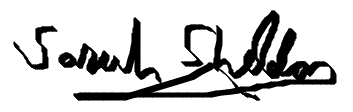
\includegraphics[height=1.1cm]{figures/coverletter_image2.png}\\[4pt]
\textbf{Sarah S.\ Sheldon}\\
Department of Psychology\\
Faculty of Science\\
University of Alberta\\
\texttt{ssheldon@ualberta.ca}
\end{minipage}

\end{document}
